\chapter{Creation of the Artifact}
\label{creation_of_the_artifact}

\section{Initial Goals}
\label{artefact_inital_goals}

As this project was first and foremost a project, designed to interactively explore the problemspace from the perspective of the \ac{HPC} community, 
all the while being contained by business requirements and time constraints, the initial goals of this project were very broad and open ended. 
At first the initial goal was simply to create a \ac{PoC} of a realistic workflow engine using the "Arkouda" project,
in order to present the Customer with a easily graspable example of its capabilities.

While we are approaching the problem from the perspective of the \ac{HPC} community, the intended enduser of this tool are the data scientists and \ac{SME}s 
that are working with the \ac{HPC} systems, and therefore the tool needs to be designed and selected with the fact in mind that the enduser will most likely not be knowledgeable in the field of \ac{HPC} or the underlying infrastructure.

In the first iteration of the project a preselection of possible Workflow management tools was given from the business side,
with the option to increase the scope if the presented tools were not sufficient.

Therefore the goals of the first iteration of this project was twofold, first to determine which, if any, of the presented tools were suitable for the task at hand,
and to determine what would make an adequate \ac{PoC} for the customer.

The following iterations are split into the tree main aspects of the project and will be discussed in their own subsections.
While these steps where happening concurrently, they each address a different aspect of the project and therefore underwent their own iterative processes.


\newpage 


\section{Overall Structure}
 
\begin{figure}[htb]
    \centering
    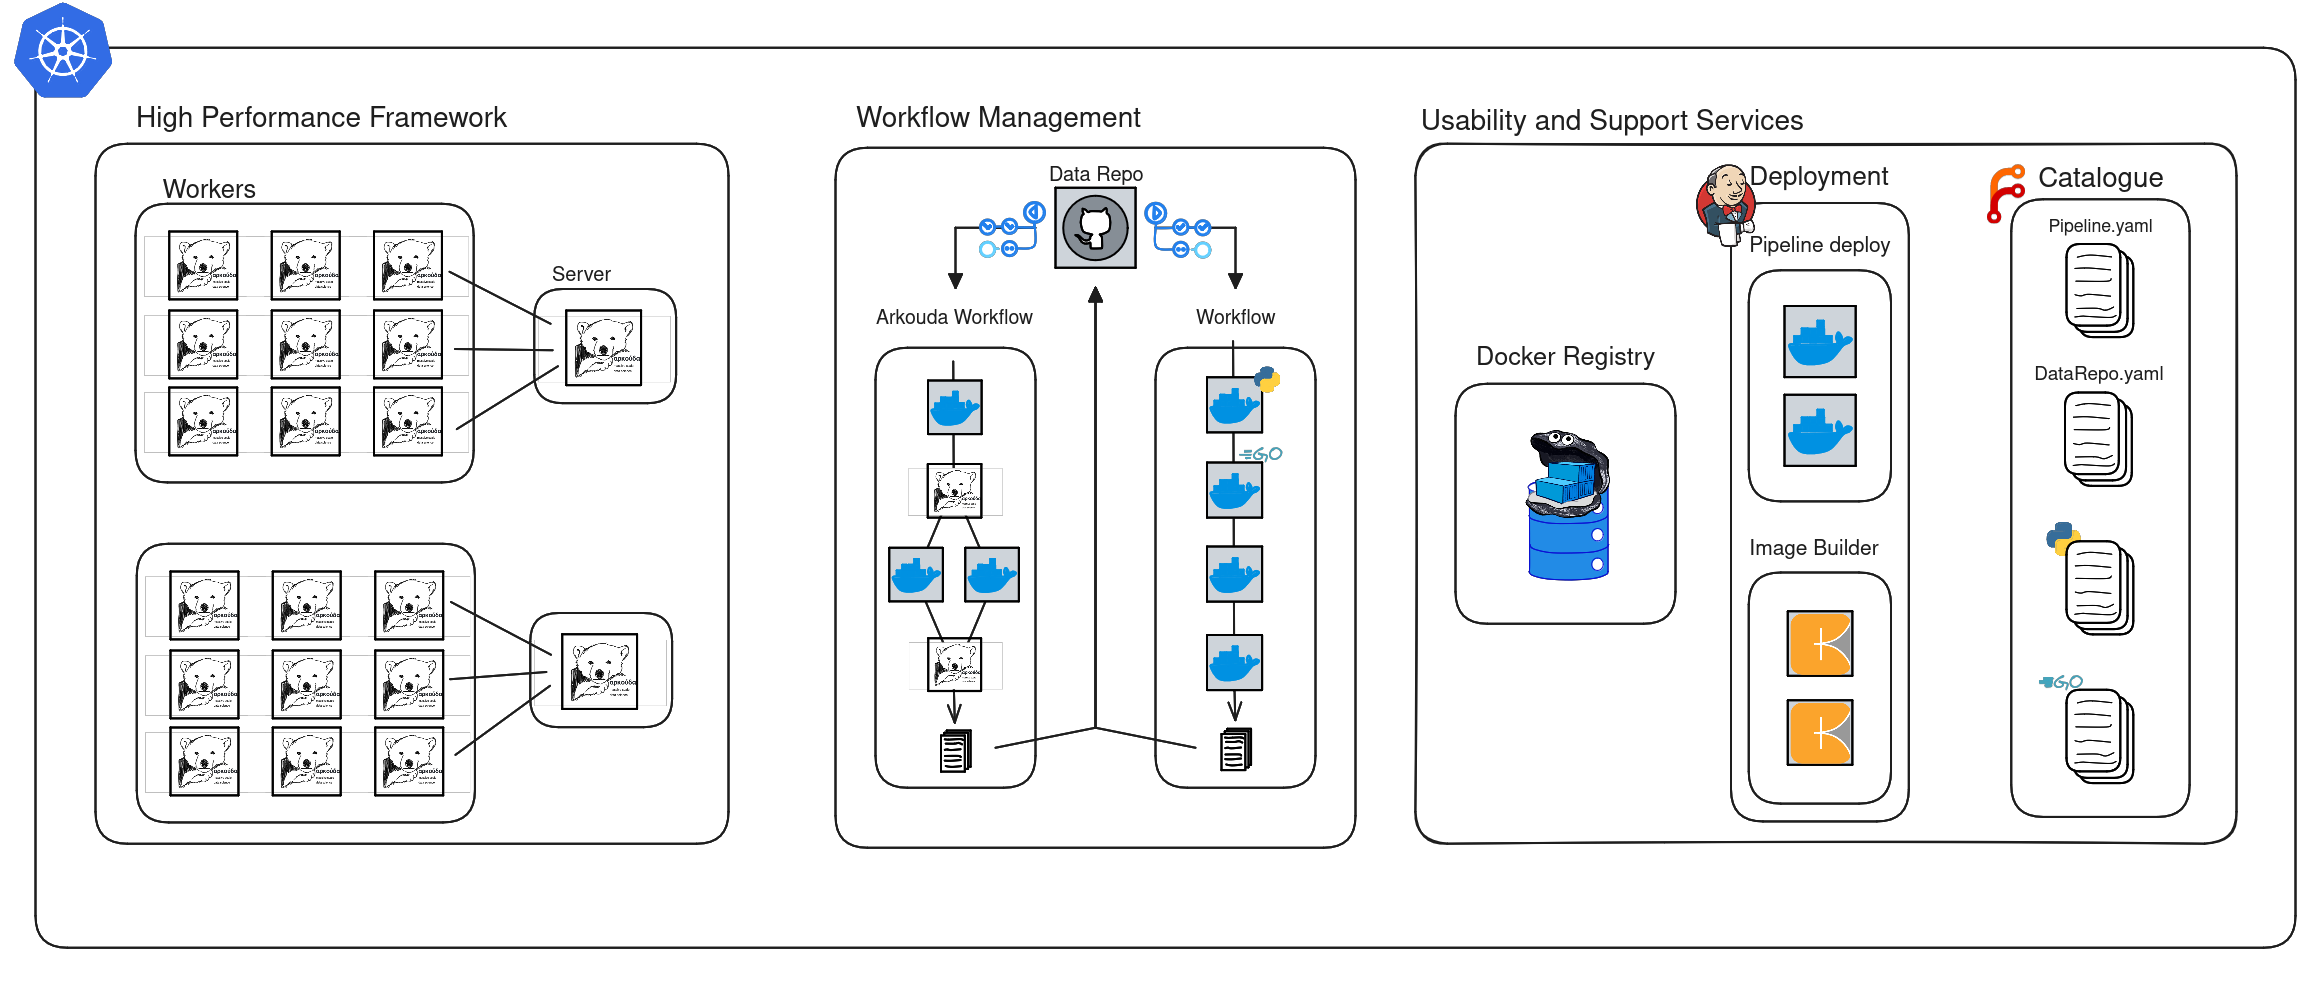
\includegraphics[width=16cm]{graphics/pachykouda_three_aspects.png}
    \caption[Pachykouda high level diagram showing three main aspects]{Pachykouda high level infrastructure diagramm}
    \label{abb:pachykouda_three_aspects}
\end{figure}


As can be seen in figure \ref{abb:pachykouda_three_aspects}, the artifact is composed of 3 main components, 
the \textbf{Central Workflow Engine} which is responsible for the orchestration of the workflows (center) and interfaces directly with the underlying infrastructure,
the \textbf{\ac{HPC} Framework} which is responsible for the execution of \ac{TCP} workloads (left)
and the \textbf{Supplementary Services} which aim at improving the usability and accessability for the enduser (right).

All this is build ontop of a hardware agnostic \ac{k8s} cluster, which is responsible for the orchestration of the different components and the underlying infrastructure.

\newpage

\section{Selection of Workflow Management Tools}

As described in section \ref{artefact_inital_goals}, the first iteration of this project was to determine which, if any, of the presented tools were suitable for the task at hand.
The following section will describe the process of selecting the tools and the criteria that were used to evaluate them.
Because the time frame does not allow for a full integration and testing of all the presented tools in depth we will be using a decision-making framework to evaluate the tools,
as described in the Methodologies \Ref{decision_making} to determine which tools will be most suitable for an initial \ac{PoC} and will serve as a good starting point for the project and future iterations.

\begin{itemize}
    \item \textbf{Pachyderm:} A \ac{k8s} based Workflow manager, written in go which was recently acquired by \ac{HPE}.
    \item \textbf{Argo:} A \ac{k8s} based Workflow manager, written in go, which is a \ac{CNCF} project \footcite{ArgoprojArgoworkflows2023}.
    \item \textbf{\ac{CLASP}:}  An in-house developed workflow manager, written in Java, utilizing Serverlet to execute workflows\footcite{sayersCloudApplicationServices2015}.
    \item \textbf{Snaplogic:} A commercial low-code/no-code workflow manager with a focus on data integration and data engineering\footcite{IPaaSSolutionEnterprise}.
\end{itemize}

But given that it was possible to select projects outside the initial selection, the following projects also need to be considered:


\begin{itemize}
    \item \textbf{Airflow:} A Python-based workflow manager under the \ac{CNCF} umbrella, known for its easy-to-use interface and extensibility\footcite{hainesWorkflowOrchestrationApache2022}.
    \item \textbf{Kubeflow:} A \ac{k8s}-native platform for deploying, monitoring, and running ML workflows and experiments, also a \ac{CNCF} project, streamlining \ac{ML} operations alongside other Kubernetes resources \footcite{Kubeflow}.
    \item \textbf{Knative:} An open-source \ac{k8s}-based platform to build, deploy, and manage modern serverless workloads, simplifying the process of building cloud-native applications \footcite{HomeKnative}.
    \item \textbf{Luigi:} An open-source Python module created by Spotify to build complex pipelines of batch jobs, handling dependency resolution, workflow management, and visualization seamlessly \footcite{SpotifyLuigi2023}.
    \item \textbf{\ac{CWL}:} An open-standard for describing analysis workflows and tools in a way that makes them portable and scalable across a variety of software and hardware environments, from workstations to cluster, cloud, and high-performance computing environments.
\end{itemize}
    
\subsubsection{Selection Criteria}

Due to this extensive list of diverse tools, a set of criteria was established to determine which tool would be the most suitable for the task at hand.
The following list of criteria was established to evaluate the tools:

\begin{itemize}
    % \item \textbf{Ease of use:} 
    %     As the hinted end users of the tool are not primarily \ac{HPC} experts, the tool needs to be easy to use and understand,
    %     and should not require the end user to have a deep understanding of the underlying infrastructure.
    %     While we can expect that the administration of the infrastructure will be done by adequately trained personnel, 
    %     the end users should be spared having to adapt to the underlying infrastructure as much as possible.

    \item \textbf{Community, Support and  Documentation:}
        Due to the limited time frame in which this project is being executed, the time to learn the intricacies of a given software is limited an important factor for this is therefore, that software needs to be adequately documented, and a support framework needs to be in place.
        Be it a community of users or a dedicated support team, the end users and the developers need to be able to rely on the software being maintained and updated as well as being able to find expert help in case of problems.

    \item \textbf{Maturity:}
        With the boom of \ac{AI} and \ac{ML} in recent years \footcite{24TopAI}, the number of tools and frameworks has exploded, and while this is a good thing it also means that a lot of these tools are still paving their way and are developing rapidly.
        While this is not necessarily a bad thing, it does mean that the tool might not be ready for production use and might not be able to provide the stability and reliability that is required for a production environment or are lacking in documentation and support.      

    \item \textbf{Strategic alignment with \ac{HPE}:}
        As this project is being developed within the context of \ac{HPE}, it is important to consider the strategic alignment of the tool with \ac{HPE}.
        \ac{HPE} has is a large company with a diverse portfolio of products and services, and this project intersects with many parts of the company.
        Therefore, it is important to consider the strategic alignment of the tool with \ac{HPE} and its products and services.

    \item \textbf{License:}
        \label{crit:license}
        While this \ac{PoC} is not a commercial product in itself but rather an exploration of the problem space and a demonstration of what a final commercial product  might be like,
        it is important to consider the licenses of the tools that are being used.
        Having to strip out a tool later on because of licensing issues would be a significant setback and therefore needs to be considered.

    \item \textbf{Cost:}
        Time is not the only constraint of this project, as the project is being developed within the context of \ac{HPE} it is important to consider the cost of the tools that are being used.

\end{itemize}

\subsubsection{Weighing of the Criteria}

An integral part of the \ac{SMART} methodology is the weighting of the criteria, as described in section \ref{decision_making}.
In order to rank the criteria themselves, as they are quite hard to quantify, 
We will be using the weighing methodology as described in the \ac{SMART-ER} methodology \ref{acro:SMART-ER}.

The first step of which is the ranking of the criteria from most important to least important.

\begin{enumerate}
    \item \textbf{ Community, Support \& Docs } This also applies for the external support available to the development team as if they are stuck, no developed can proceed, no matter the other factors.
    \item \textbf{ License } This criterion has to weighted carefully, as a highly restrictive license might be a deal-breaker, but a license that is too permissive might conflict with the strategic alignment with \ac{HPE}.
    \item \textbf{ Strategic alignment with \ac{HPE} } As this is developed by and for \ac{HPE} their requirements need to be considered as well.
    % \item \textbf{ Ease of Use } While the ease of use is important as this should eventually become a product, for now the central aspect is to create a \ac{PoC} therefore the usability is a priority, but not the highest.
    \item \textbf{ Cost } As this is a \ac{PoC} and not a commercial product, the cost is not the highest priority as this will be of small scale and therefore the cost will be negligible in most cases.
    \item \textbf{ Maturity } While the maturity of the tool is important, as this is a \ac{PoC} and not a commercial product, if the maturity of the tool does not impact the extensibility of the tool or the development process, it is not the highest priority.
\end{enumerate}

As all these criteria are quite important, the weighting function selected for the criteria is the \ac{RS} function, as described in section \ref{smart_er}, 
as it does not rank the criteria too harshly.
The lookup tables for the weighting function can be found in the appendix \ref{abb:pipeline_communication_sld}.

\begin{table}[htb]
    \centering
    \begin{tabular}{|l|l|} \hline
        \textbf{Criteria}                       & \textbf{Weight}       \\ \hline
        Community, Support and  Documentation   &  0.3333               \\ \hline
        License                                 &  0.2667               \\ \hline
        Strategic alignment with \ac{HPE}       &  0.2000               \\ \hline
        % Ease of use                             &  0.1071               \\ \hline
        Maturity                                &  0.1333               \\ \hline
        Cost                                    &  0.0667               \\ \hline
    \end{tabular}
    \caption{Weighting of the criteria}
    \label{tab:weighting_of_the_criteria}
\end{table}

\subsubsection{Evaluation of the Tools}

Now that we have established the criteria as well as their weighing, we can begin to evaluate the tools based on the criteria.
Here we will be using a mix of Methodologies, as some of these criteria can simply be indexed via analogous values, while others are of a more non-specific nature.
The discussion of which values will be used on which weighing scale for the tools' comparison can be found in the appendix in the sections 1 - 5 \ref{tool_eval}


\begin{table}[htb]
    \centering
    \begin{tabular}{|l|l|l|l|l|} \hline
        \textbf{Criteria}                                          & \textbf{Pachyderm}    & \textbf{Argo}         & \textbf{\ac{CLASP}}   & \textbf{Snaplogic}     \\ \hline
        % Ease of use                                                & TBD                   & TBD                   & TBD                   & TBD                    \\ \hline
        Community, Support \& Docs                                 & 8.43                   & 2.32                   & 2.5                   & 5.03                   \\ \hline
        Maturity                                                   & 7.86                 & 5.2                   & 2.5                   & 5                   \\ \hline
        Strategic alignment                                        & 10                   & 2.5                   & 7.5                   & 0                    \\ \hline
        License                                                    & 10                    & 7.5                     & 10                    & 0                      \\ \hline
        Cost                                                       & 6                      & 10                    & 10                    & 3                      \\ \hline
    \end{tabular}
    \caption{Evaluation of the suggested tools}
    \label{tab:evaluation_of_the_suggested_tools}
\end{table}

The following table shows the evaluation of the tools which where chosen for their relevance to the problem space, based on the criteria and the weighting of the criteria:

\begin{table}[htb]
    \centering
    \begin{tabular}{|l|l|l|l|l|l|} \hline
        \textbf{Criteria}                                          & \textbf{Airflow}      & \textbf{Kubeflow}     & \textbf{Knative}      & \textbf{Luigi}        & \textbf{CWL}          \\ \hline
        % Ease of use                                                & TBD                   & TBD                   & TBD                   & TBD                   & TBD                   \\ \hline
        Community, Support \& Docs                                 & 10                    & 2.25                  & 0.74                  & 2.29                  & 0.22                  \\ \hline
        Maturity                                                   & 9.41                  & 5.05                  & 6.43                  & 5.23                  & 3.98                  \\ \hline
        Strategic alignment                                        & 2.5                   & 2.5                   & 2.5                   & 2.5                   & 2.5                   \\ \hline
        License                                                    & 7.5                   & 7.5                   & 7.5                   & 7.5                   & 7.5                   \\ \hline
        Cost                                                      & 10                    & 10                    & 10                    & 10                    & 10                    \\ \hline

    \end{tabular}
    \caption{Evaluation of the additional tools}
    \label{tab:evaluation_of_the_additional_tools}
\end{table}

\subsubsection{Conclusion of the Selection Process}

Now we can use these values and the weighting of the criteria to calculate the overall score of the tools, in order to find out which tool is the most suitable for the task at hand.
The following table shows the overall score of the tools:

\begin{table}[H]
\centering
\begin{tabular}{|l|l|} \hline
    \textbf{Tool} & \textbf{Score} \\ \hline
    Pachyderm     & 8.9247         \\ \hline
    Airflow       & 7.7546         \\ \hline
    CLASP         & 6.0005         \\ \hline
    Argo          & 4.6337         \\ \hline
    Luigi         & 4.6277         \\ \hline
    Kubeflow      & 4.5903         \\ \hline
    Knative       & 4.2710         \\ \hline
    CWL           & 3.7711         \\ \hline
    Snaplogic     & 2.5431         \\ \hline
\end{tabular}
\caption{Overall score of the tools}
\label{tab:overall_score_of_the_tools}
\end{table}


As can be seen in table \ref{tab:overall_score_of_the_tools}, Pachyderm emerged as the most suitable tool, with the highest overall score of 8.9247. 
This suggests that Pachyderm aligns well with the project's goals and the requirements of HPE, thanks to its strong community support, documentation, and strategic alignment with HPE's objectives.

Airflow followed Pachyderm with a score of 7.7546, indicating its strength in community support and documentation, as well as its cost-effectiveness.
Although Airflow did not score as high as Pachyderm, it remains a strong contender for use in future iterations of the project.

CLASP, an in-house developed tool, had a moderate score of 6.0005, which might make it suitable for initial\ac{PoC} phases due to its alignment with the existing ecosystem and its no-cost advantage.
However, its lower scores in other criteria might limit its potential for broader implementation.

Argo, Luigi, Kubeflow, and Knative scored in the middle range,
suggesting they could be considered for specific use cases but may not be as well-rounded for the project's current needs as Pachyderm or Airflow.

CWL's lower score of 3.7711 indicates it may not meet the project's requirements as effectively as the other tools evaluated.
Its lower score in community support and strategic alignment with HPE's goals could be areas of concern.

Lastly, Snaplogic scored the lowest at 2.5431, suggesting that it may not be well-suited for this project's objectives,
especially given its lack of a strong strategic alignment with HPE and lower scores in community support and documentation. 



\section{Implementation of the Artifact}

This section will describe the iterative process of implementing the larger artifact and is broken up into 3 subsections.
While these steps where happening concurrently, they each address a different aspect of the project and therefore underwent their own iterative processes.



\subsection{Infrastructure}


\subsubsection{First iteration - Minikube}
As the decision of the Workflow management tool was made, it was obvious that a dedicated \ac{k8s} infrastructure was needed to run the tool\footcite{PachydermDocsOnPrem}.
The Pachyderm documentation gave two recommendations for setting up an initial development environment, preferably Docker Desktop or alternatively Minikube \footcite{PachydermDocsLocal}.
Due to the exclusive license of Docker-Desktop\footcite{DockerTermsService2022},
which prevents large companies free usage of the product\footcite{DockerFAQsDocker2021} the choice fell on Minikube for an initial test setup.

In addition to the underlying \ac{k8s} Pachyderm also needs an external S3 Storage Bucket for its \ac{PFS} for which we used MinIO,
a self hostable S3 compliant object storage\footcite{incMinIOMinIOKubernetes}, which was also based on recommendations by the Pachyderm documentation.

The persistent storage requirements for the Pachyderm itself was fulfilled by manually creating two \ac{PV}'s on the hosts local harddrive.
Using the Helm packagemanager\footcite{HelmDocsHome} for \ac{k8s} the at that point newest version 2.6.4 was installed from the official Artifacthub repository\footcite{ArtifacthubPachyderm}.

The hostsystem of this iteration was a single ProLiant DL385 Gen10 Plus running Ubuntu 22.04.3 LTS x86\_64.
During the setup every step was diligently noted and put into a repository\footcite{eckerthInstallationInstructionsMinikube}, alongside the needed scripts. 
The instructions can be found in the appendix at \ref{appendix:minikube_installation_instructions}.


\subsubsection*{Learnings from the first iteration}

The shortcomings of this naive first iteration became apparent very quickly, 
which was to be expected, as the goal of this iteration was to create a minimal working example to get a better understanding of the toolings and the underlying infrastructure.

The first and foremost issue where the limitations imposed by Minikubes reliance on an Internal \ac{VM},
during testing the inability to on the fly increase the resources of the \ac{VM} became a significant bottleneck.
At some point during the testing of \ref{tcpp_hpc_workloads} the \ac{VM} was so overloaded that the installation was irreparably damaged which was seen as a sign to move on to the next iteration.

Another more subtle issue was the discrepancy between the experience a small scale \ac{k8s} installation within Minikube and a large scale \ac{k8s} cluster like the one that would be used in later steps of the project.
Therefore it was decided that a more realistic \ac{k8s} cluster would be needed for the next iteration, which became the Heydar cluster.

\subsubsection{Second iteration - Heydar Cluster}
\label{heydar_cluster}

Improving upon the shortcomings of the first iteration, the second iteration was based in the attempt to create a more realistic \ac{k8s} cluster.
To achieve this 20 ProLiant DL360 Gen9 Servers, running Ubuntu 22.04.3 LTS x86\_64 where used to create a bare metal \ac{k8s} cluster,
using kubeadm as it provides deep integration with the underlying infrastructure\footcite{CreatingClusterKubeadm}.

But a bare metal cluster also comes with its own set of challenges, as the cluster needs to be provisioned and configured manually.
In order to automate this process, the Ansible automation tool was used to set up all the nodes in praralel and to ensure that the all the nodes are in the same state.
Ansible is a declarative tool which allows for the automation of the provisioning and configuration of the cluster\footcite{Ansible2023}, by specifying the desired state of the cluster in a playbook and then applying it to the cluster.
The Ansible playbook used for the setup of the cluster can be found at \ref{appendix:ansible_setup_script}.

Which unknowingly caused conflict between the Ansible playbook and the maintenance scripts of the cluster as the Heydar machines.
As \ac{k8s} needs very specific configurations on the underlying infrastructure like the deactivation of swap space\footcite{InstallingKubeadm}.

This was resolved by consulting with the maintainer of the cluster and adjusting the Ansible playbook as well as the maintenance config for the cluster nodes accordingly, 
after we had identified the issue.


One important aspect of a production like cluster is the networking, as \ac{k8s} does not natively manage communication on a cluster level,
but instead relies on so called \ac{CNI}s to manage and abstract the underlying network infrastructure \footcite{ClusterNetworking}.

Here we where spoiled for choice once again, as there are a multitude of different \ac{CNI}s available, each with their own advantages and disadvantages.
The Kubernetes documentation provides a non exhaustive list of 17 different \ac{CNI}s\footcite{KubernetesCNIPlugins}, which all fulfill this essential task in different ways.
As the needs regarding the network plugin where not very specific at this point, the choice fell on Calico, as surface level research showed that it was a popular choice for bare metal clusters\footcite{ExploreNetworkPlugins},
provided security and enterprise support as well having a wide range of features\footcite{mehndirattaComparingKubernetesContainer}.
But Calico proved to be more difficult to setup than expected, after consulting with a college who set up a different cluster with Calico,
it was decided to use Flannel as a \ac{CNI} instead.
Flannel turned out to be much easier to setup and configure, as it is a very lightweight \ac{CNI} which is designed for bare metal clusters\footcite{Flannel2023}, 
and foregoes the more advanced security features of Calico. 

The Flannel configuration used for the cluster can be found at \ref{appendix:flannel_config} it is closely based on the example configuration provided by the Flannel documentation\footcite{FlannelInstallConfig}.

\subsubsection*{Learnings from the second iteration}

The second iteration was a significant improvement over the first iteration, as it provided a much more realistic environment for the development of the artifact.
But it also came with its own set of challenges, as the bare metal cluster needed to be provisioned and configured manually, which was a significant time investment.

What became apparent very quickly was that the solution for the provisioning of the \ac{PV} was no where near scalable,
as it relies on the local harddrive of the host machine and therefore must host the container on the same machine as the \ac{PV} which defeats the purpose of a multi node cluster in the first place.
Therefore a more scalable solution needs to be implemented for the next iteration.
A possible solution could be the use of distributed storage solutions like Ceph\footcite{CephIoHome} or GlusterFS\footcite{Gluster}  in combination with the Rook project \footcite{Rook}. 
which will need to be explored in future iterations.


As described in section XXX a service hosting \ac{FAM} will be needed in future iterations aswell.

\subsection{\ac{TCPP} HPC Workloads} 
\label{tcpp_hpc_workloads}

\subsection{Supplementary Services}



\newpage    


\section{Evaluation of the Artifact}

\newpage
